\documentclass[11pt, a4paper]{article}
%\usepackage{geometry}
\usepackage[inner=1.5cm,outer=1.5cm,top=2.5cm,bottom=2.5cm]{geometry}
\pagestyle{empty}
\usepackage{graphicx, multicol}
\usepackage{fancyhdr, lastpage, bbding, pmboxdraw}
\usepackage[usenames,dvipsnames]{color}
\definecolor{darkblue}{rgb}{0,0,.6}
\definecolor{darkred}{rgb}{.7,0,0}
\definecolor{darkgreen}{rgb}{0,.6,0}
\definecolor{red}{rgb}{.98,0,0}
\usepackage[colorlinks,pagebackref,pdfusetitle,urlcolor=darkblue,citecolor=darkblue,linkcolor=darkred,bookmarksnumbered,plainpages=false]{hyperref}
\renewcommand{\thefootnote}{\fnsymbol{footnote}}


\pagestyle{fancyplain}
\fancyhf{}
\lhead{ \fancyplain{}{GRSC 7770} }
%\chead{ \fancyplain{}{} }
\rhead{ \fancyplain{}{\today} }
%\rfoot{\fancyplain{}{page \thepage\ of \pageref{LastPage}}}
\fancyfoot[RO, LE] {page \thepage\ of \pageref{LastPage} }
\thispagestyle{plain}

%%%%%%%%%%%% LISTING %%%
\usepackage{listings}
\usepackage{caption}
\DeclareCaptionFont{white}{\color{white}}
\DeclareCaptionFormat{listing}{\colorbox{gray}{\parbox{\textwidth}{#1#2#3}}}
\captionsetup[lstlisting]{format=listing,labelfont=white,textfont=white}
\usepackage{verbatim} % used to display code
\usepackage{fancyvrb}
\usepackage{acronym}
\usepackage{amsthm}
\VerbatimFootnotes % Required, otherwise verbatim does not work in footnotes!



\definecolor{OliveGreen}{cmyk}{0.64,0,0.95,0.40}
\definecolor{CadetBlue}{cmyk}{0.62,0.57,0.23,0}
\definecolor{lightlightgray}{gray}{0.93}



\lstset{
%language=bash,                          % Code langugage
basicstyle=\ttfamily,                   % Code font, Examples: \footnotesize, \ttfamily
keywordstyle=\color{OliveGreen},        % Keywords font ('*' = uppercase)
commentstyle=\color{gray},              % Comments font
numbers=left,                           % Line nums position
numberstyle=\tiny,                      % Line-numbers fonts
stepnumber=1,                           % Step between two line-numbers
numbersep=5pt,                          % How far are line-numbers from code
backgroundcolor=\color{lightlightgray}, % Choose background color
frame=none,                             % A frame around the code
tabsize=2,                              % Default tab size
captionpos=t,                           % Caption-position = bottom
breaklines=true,                        % Automatic line breaking?
breakatwhitespace=false,                % Automatic breaks only at whitespace?
showspaces=false,                       % Dont make spaces visible
showtabs=false,                         % Dont make tabls visible
columns=flexible,                       % Column format
morekeywords={__global__, __device__},  % CUDA specific keywords
}

%%%%%%%%%%%%%%%%%%%%%%%%%%%%%%%%%%%%
\begin{document}
\begin{center}
{\Large \textsc{GRSC 7770 Graduate Teaching Seminar}}
\end{center}
\begin{center}
Fall 2018
\end{center}
% \date{September 26, 2014}


\begin{center}
\rule{6in}{0.4pt}
\begin{minipage}[t]{.75\textwidth}
\begin{tabular}{llcccll}
\textbf{Instructor:} & William E. Olsen & & &  & \textbf{Time:} & R 3:30 -- 4:45pm \\
\textbf{Email:} &  \href{mailto:wolsen@uga.edu}{wolsen@uga.edu} & & & & \textbf{Place:} & 303 Boyd Graduate Studies
\end{tabular}
\end{minipage}
\rule{6in}{0.4pt}
\end{center}
\vspace{.5cm}
\setlength{\unitlength}{1in}
\renewcommand{\arraystretch}{2}


\noindent\textbf{Course Webpage:} eLC

\vskip.15in
\noindent\textbf{Office Hours:} After class, or by appointment.

\vskip.15in
\noindent\textbf{Main References:} %\footnotemark
This is a restricted list of useful books that will be touched on during the course. You need to consult them occasionally.
\begin{itemize}
\item The {\textit{MAA Instructional Practices Guide}}.
\item Steven G. Krantz, {\textit{How to Teach Mathematics}}, American Mathematical Society, 1991.
\end{itemize} 

% \footnotetext{Downloadable ebook versions are available on AeLP.}
\vskip.15in
\noindent\textbf{Course Description:}
The primary goal of this seminar is to prepare graduate students for their roles as teaching assistants (and graduate student teachers) in the Department of Mathematics. A portion of the seminar will be devoted to department and university policies and procedures related to teaching. We will also discuss the roles that teaching assistants play in the department and how to balance that role with other responsibilities. Most importantly, we study and discuss effective teaching practices for undergraduates and why these practices are important in both academic and professional positions. 

\vskip.15in
\noindent\textbf{Specific learning goals:}
We will use a variety of formats (e.g., small-group-discussion, presentations) to explore the ins and outs of teaching mathematics as a graduate student.  By the end of this course you will be introduced to:
\begin{multicols}{2}
\begin{itemize}
\item how to set the stage for your first class.
\item motivation in the college classroom.
\item assessments and rubrics.
\item teaching culturally diverse students.
\item dealing with student problems and problem students.
\item inquiry-based learning.
\item teaching controversial issues.
\item teaching opportunities at UGA.
\end{itemize}
\end{multicols}

\vspace*{.15in}
\noindent\textbf{Grading Policy:}  Course grades will be assigned as either $S/U$ (Satisfactory/Unsatisfactory). To receive an $S$, students must:
\begin{itemize}
\item Complete all required readings and assignments.
\item Participate in class and provide peer feedback.
\item Have no more than two unexcused absences.
\end{itemize}

\vskip.15in
\noindent\textbf{Communication:}
To comply with the Family Educational Rights and Privacy Act (FERPA), all communication that refers to individual students must be through a secure medium (UGAMail or eLC) or in person. Instructors are not allowed to respond to messages that refer to individual students or student progress in the course through non-UGA accounts, phone calls, or other types of electronic media.

\vskip.15in
\noindent\textbf{Academic Honesty:}  It is each student’s responsibility to be familiar with University policy on academic honesty (read \textit{A Culture of Honesty: Policies and Procedures on Academic Honesty}). See \href{http://www.uga.edu/honesty/ahpd/culture_honesty.htm}{\url{http://www.uga.edu/honesty/ahpd/culture_honesty.htm}}. Any evidence of academic dishonesty will be turned over to the Office of the Vice President for Academic Affairs, for consideration and possible action.  All students have the right to appeal any decision following the appeals process outlined in \textit{A Culture of Honesty}.

\vskip.15in
\noindent\textbf{Disabilities:}
I am happy to accommodate any documented disabilities.  If you are eligible for accommodation please contact me early in the semester with proper documentation from Disability Services.  Contact Disability Services (542-8710) about requesting accommodations.

\begin{figure}[H]
  \centering
  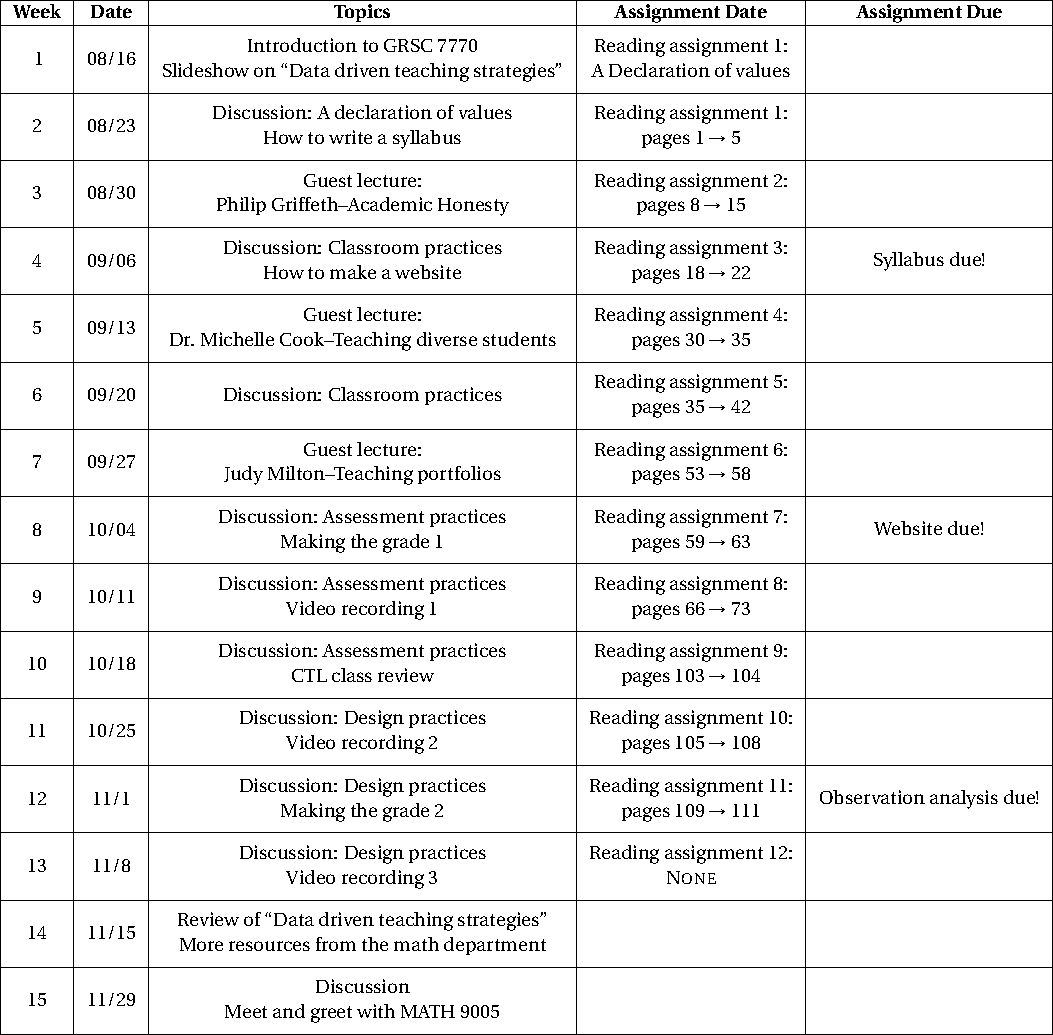
\includegraphics{SyllabusCalendar.pdf}
\end{figure}

\end{document} 
              
%%% Local Variables:
%%% mode: latex
%%% TeX-master: t
%%% End:
